\documentclass{article}
\usepackage{graphicx}
\title{Labwork 2: Get to Know Your GPU}
\author{DAO HOANG DUNG \\ Student ID: 2540047}
\date{\today}

\begin{document}

\maketitle

\section{Objective}
For this labwork, the main goal is to use numba.cuda to get to know my GPU
\begin{itemize}
     \item Devicename 
     \item Coreinfo:multiprocessorcount,corecount
     \item Memoryinfo:memorysize
\end{itemize}

\section{Python code}
\begin{figure}[htbp]
    \centering
    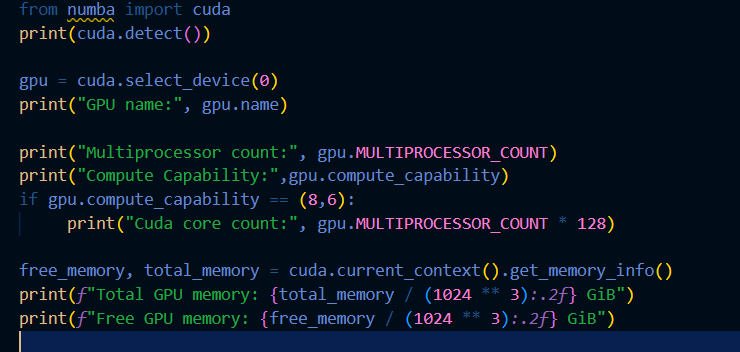
\includegraphics[width=\linewidth]{images/code.png}
    \caption{Code}
    \label{fig:gpu-output}
\end{figure}


\section{Results}
\begin{figure}
    \centering
    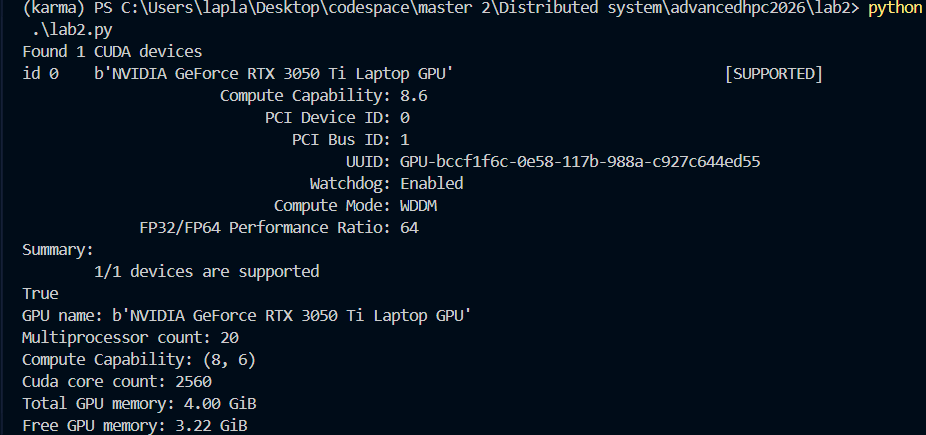
\includegraphics[width=\linewidth]{images/result.png}
\end{figure}

\end{document}
